\def\annoBubbleRadius{1cm}

\subtikzpicturedef{subCADExhaustEMODE} {
    origin%
} {
    \draw (#1-start) coordinate (#1-origin);

    \draw
    (#1-origin)
    node (#1-imgTop) [
        inner sep = 0pt,
        anchor = center,
    ] {
        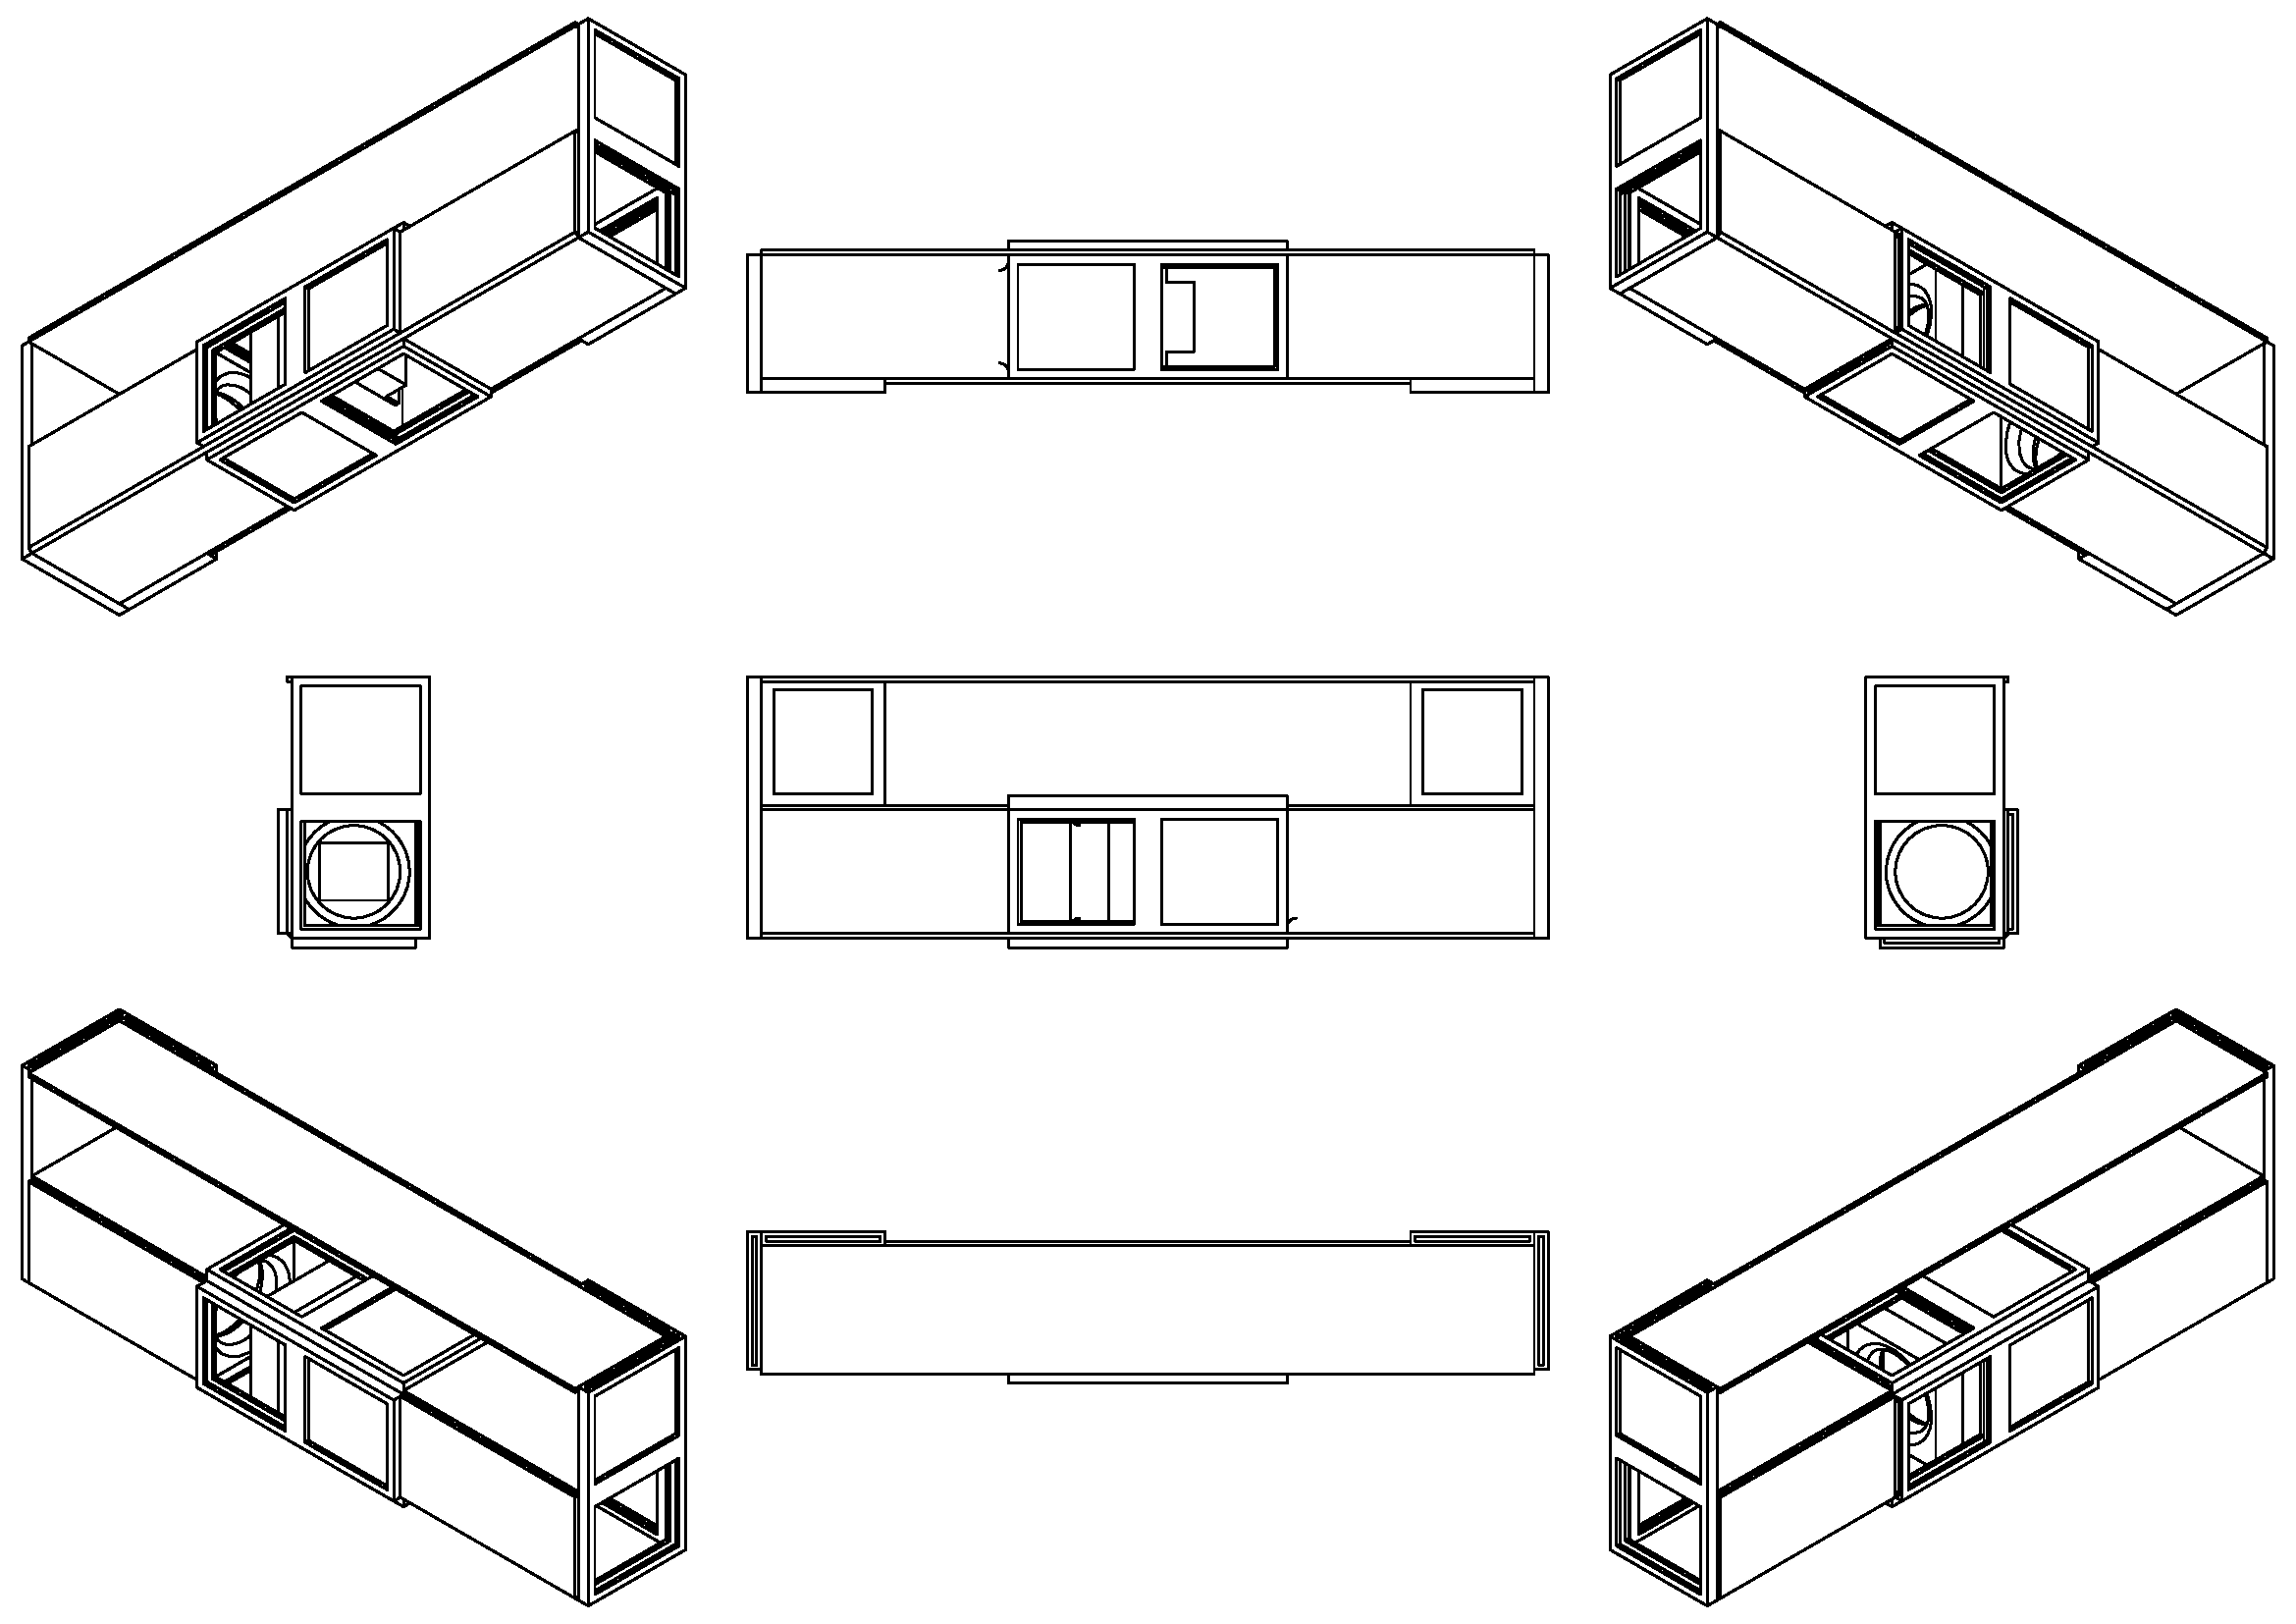
\includegraphics [
        ] {\subfix{pics/emode_top.pdf}}
    }

    (#1-imgTop.south) ++(0, -1cm)
    node (#1-imgBot) [
        inner sep = 0pt,
        anchor = north,
    ] {
        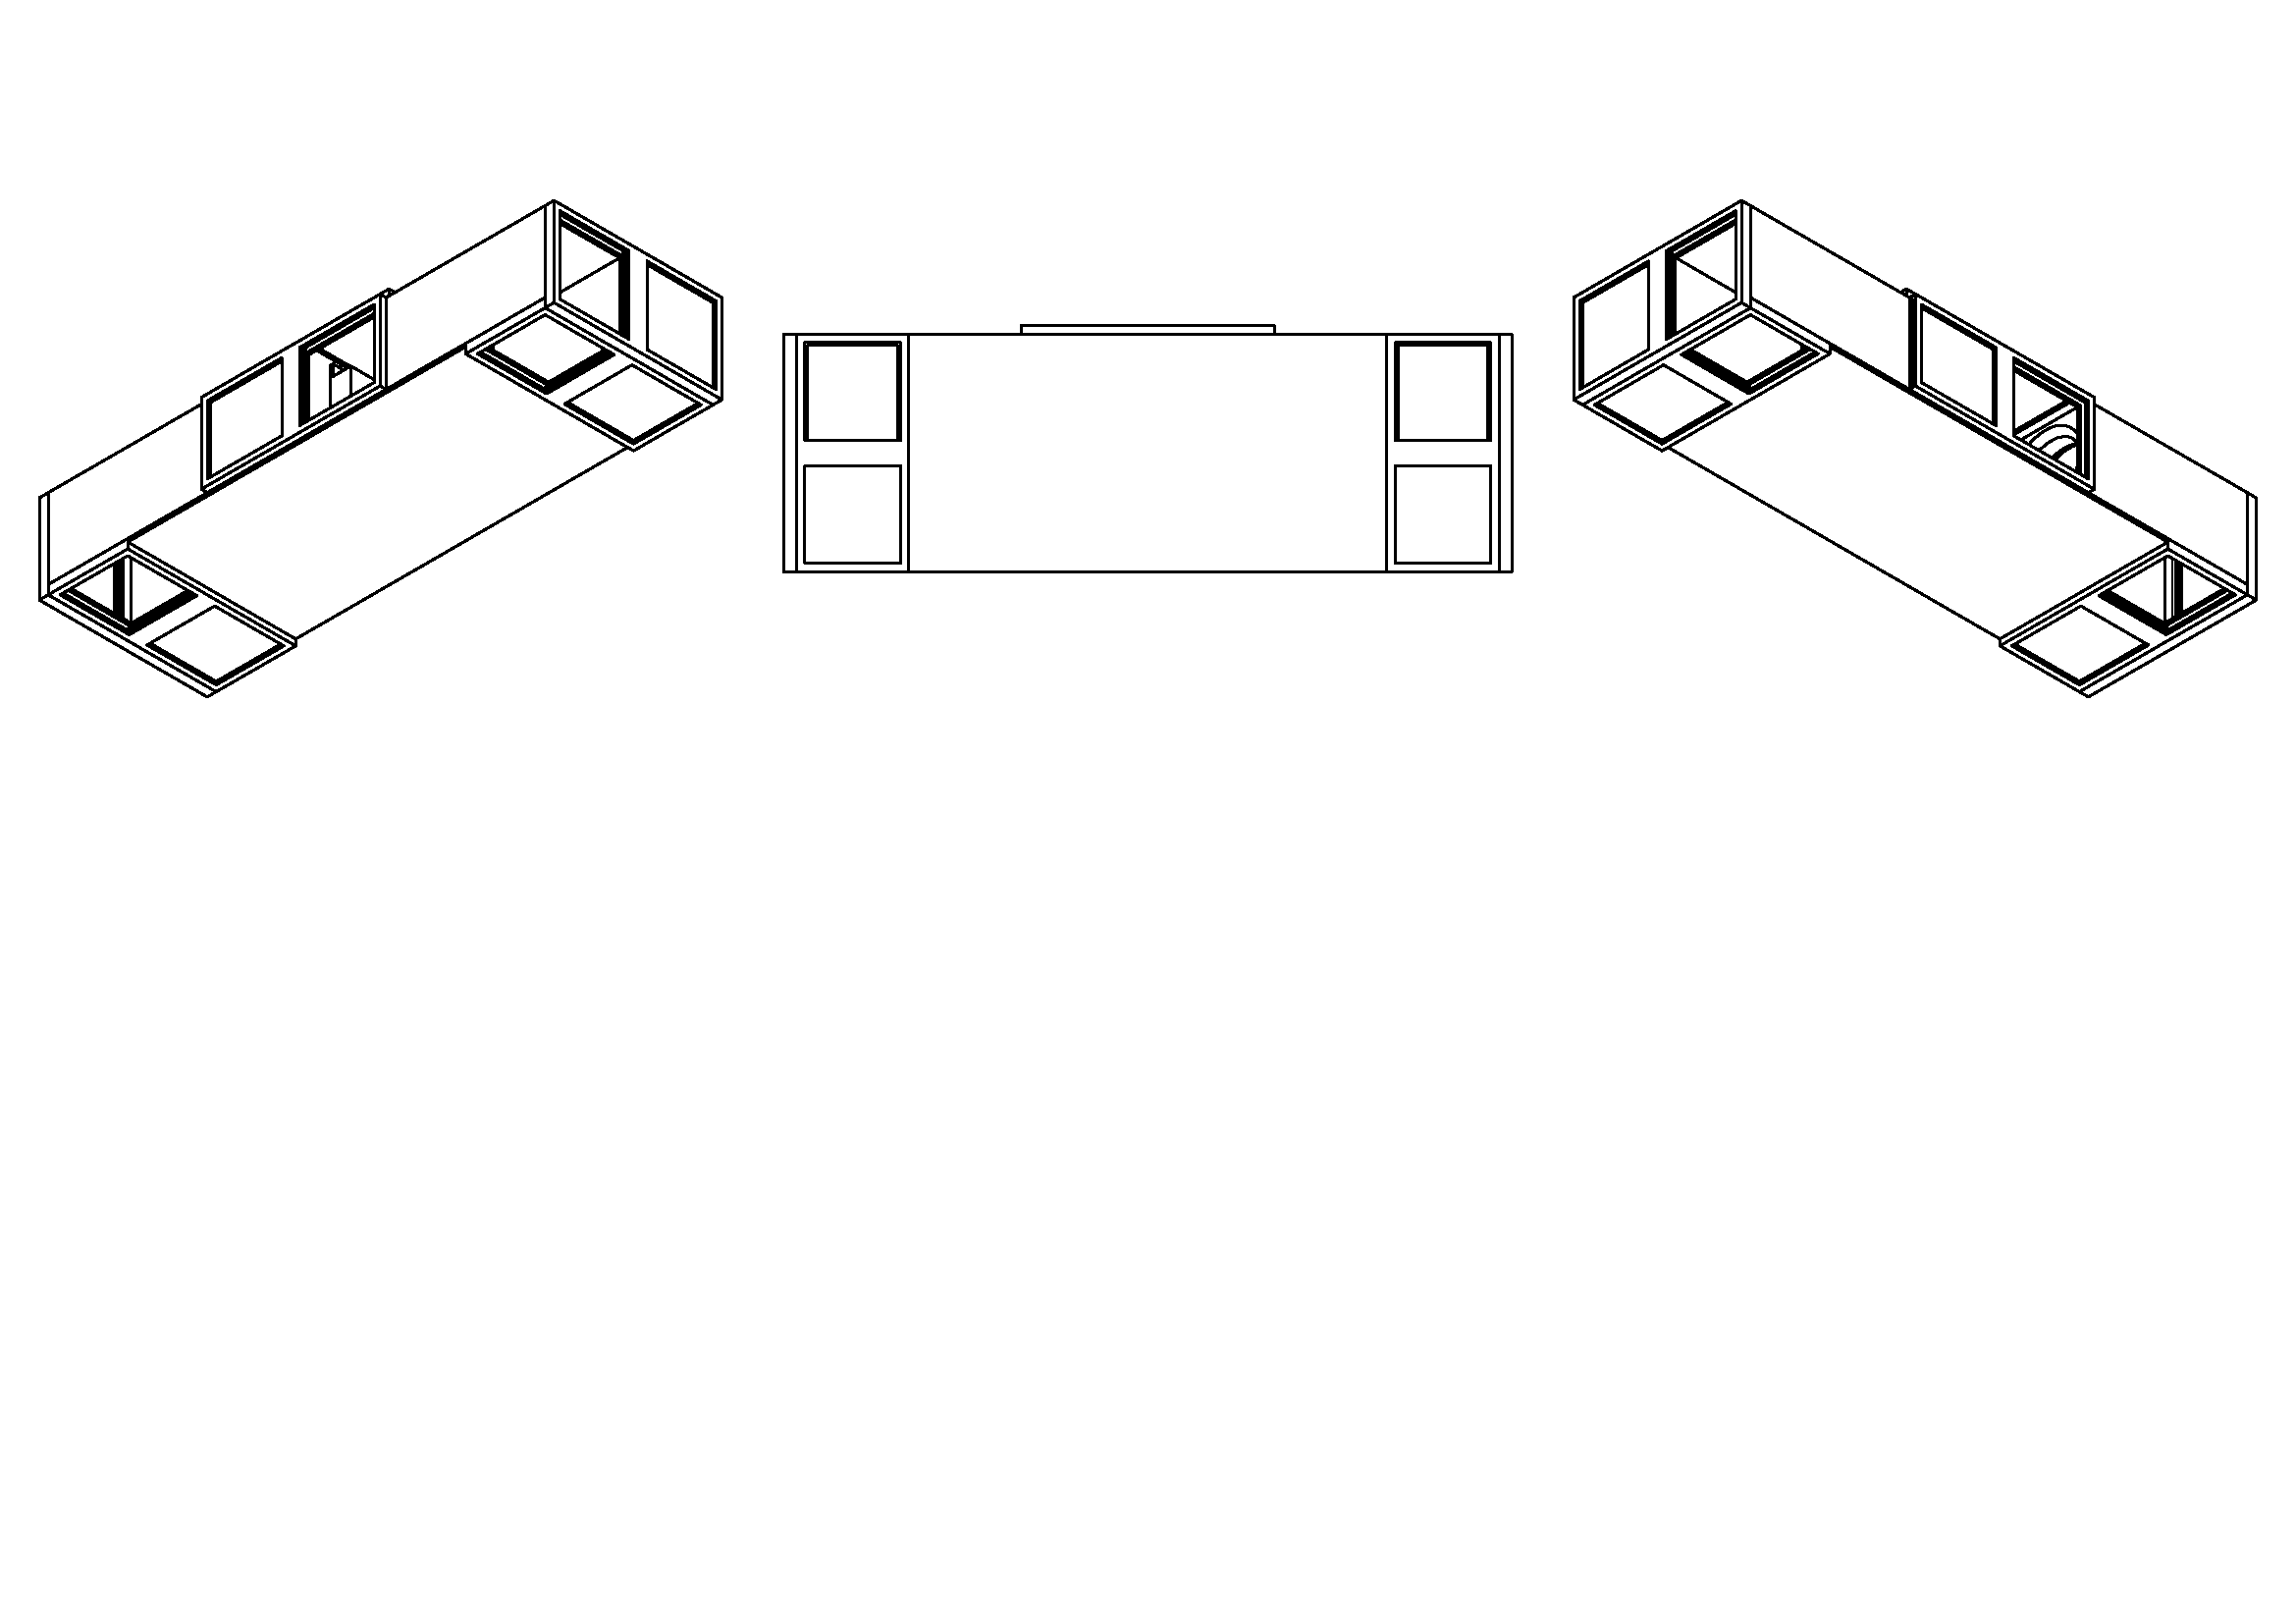
\includegraphics [
            trim = {0 16.0cm 0 3.15cm},
            clip,
        ] {\subfix{pics/emode_bot.pdf}}
    }
    ;

    %% annotation bubbles

    \draw
    (#1-imgTop.north west) ++(2.5cm, -2.0cm) coordinate (#1-bOne)
    (#1-imgTop.north east) ++(-2.5cm, -2.0cm) coordinate (#1-bThree)

    (#1-imgTop.south west) ++(2.5cm, 2.0cm) coordinate (#1-bSeven)
    (#1-imgTop.south east) ++(-2.5cm, 2.0cm) coordinate (#1-bNine)

    (#1-imgBot.north west) ++(2.5cm, -1.5cm) coordinate (#1-bTen)
    (#1-imgBot.north east) ++(-2.5cm, -1.5cm) coordinate (#1-bTwelve)

    (#1-imgTop.west) ++(2.5cm, 0) coordinate (#1-bFour)
    (#1-imgTop.east) ++(-2.5cm, 0) coordinate (#1-bSix)

    (#1-imgTop.north) ++(0, -2.0cm) coordinate (#1-bTwo)
    ($(#1-imgTop.center)!0.5!(#1-imgTop.north)$) ++(0, -2.5cm) coordinate (#1-bFive)

    (#1-imgTop.south) ++(0, 2.0cm) coordinate (#1-bEight)

    (#1-imgBot.south) ++(0, 0.0cm) coordinate (#1-bEleven)
    ;


    \foreach \coord/\bubble in {
        #1-bEleven/11,
        #1-bEight/08,
        #1-bTwo/02,
        #1-bFive/05,
        #1-bFour/04,
        #1-bSix/06,
        #1-bTen/10,
        #1-bTwelve/12,
        #1-bSeven/07,
        #1-bNine/09,
        #1-bThree/03,
        #1-bOne/01%
    } {
        \draw [
            ultra thick,
        ]
        (\coord)
        node [
            font = \huge,
        ] {
            \texttt{\bubble}
        }
        (\coord) circle (\annoBubbleRadius)
        ;
    }


    %% heading

    \draw [
        ultra thick,
    ]
    (#1-imgTop.north west) ++(0, 1) coordinate (#1-tmp)
    % (#1-tmp) -- (#1-imgTop.north east |- #1-tmp)

    (#1-tmp -| #1-imgTop.east) ++(0, 0.75cm)
    node (#1-title) [
        anchor = south east,
        % above = 1cm,
        font = \Huge,
    ] {
        \texttt{CORE BLOCK IN EMODE}
    }

    ;


    %%

    \draw
    (#1-imgBot.south east) ++(0, -1cm) coordinate (#1-tmp)

    (#1-tmp)
    node (#1-views) [
        anchor = north east,
        font = \Huge,
    ] {
        \begin{minipage} {10cm}
            \begin{tabularx} {\textwidth} {
                    >{\raggedleft \arraybackslash \ttfamily}X
                }

                DIFFERENT VIEWS \\

            \end{tabularx}
        \end{minipage}
    }

    (#1-views.south -| #1-imgBot.west) ++(0, -1cm) coordinate (#1-tmp)

    (#1-tmp)
    node (#1-annoFirst) [
        anchor = north west,
        font = \Huge,
    ] {
        \begin{minipage} {15cm}
            \renewcommand\arraystretch{1}
            \begin{tabularx} {\textwidth} {
                    >{\raggedright \arraybackslash \ttfamily}X
                }

                01 - BACK TOP LEFT\\
                04 - LEFT \\
                07 - FRONT TOP LEFT \\
                10 - BACK BOTTOM LEFT \\

            \end{tabularx}
        \end{minipage}
    }

    (#1-annoFirst.north -| #1-imgBot.south) coordinate (#1-tmp)

    (#1-tmp)
    node (#1-annoSecond) [
        anchor = north,
        font = \Huge,
    ] {
        \renewcommand\arraystretch{1}
        \begin{tabular} {
                % >{\raggedright \arraybackslash \ttfamily}X
                l
            }

            \texttt{02 - BACK} \\
            \texttt{05 - TOP} \\
            \texttt{08 - FRONT} \\
            \texttt{11 - BOTTOM} \\

        \end{tabular}
        % \begin{minipage} {6cm}
        % \end{minipage}
    }

    (#1-annoFirst.north -| #1-imgBot.east) coordinate (#1-tmp)

    (#1-tmp)
    node (#1-annoThird) [
        anchor = north east,
        font = \Huge,
    ] {
        \begin{minipage} {15cm}
            \renewcommand\arraystretch{1}
            \begin{tabularx} {\textwidth} {
                    >{\raggedleft \arraybackslash \ttfamily}X
                }

                BACK TOP RIGHT - 03 \\
                RIGHT - 06 \\
                FRONT TOP RIGHT - 09 \\
                BACK BOTTOM RIGHT - 12 \\

            \end{tabularx}
        \end{minipage}
    }

    (#1-annoFirst.south west) ++(0,-1) coordinate (#1-tmp)

    (#1-tmp)
    node (#1-note) [
        anchor = north west,
        font = \Huge,
    ] {
        \ttfamily
        NOTE: IN THIS MODE THE STATE OF MIDDLE PANELS ARE NOT THAT SIGNIFICANT.
    }

    ;

}

\subtikzpictureactivate{subCADExhaustEMODE}
